\documentclass[a4paper,11pt]{article}

\usepackage{graphicx}
\usepackage{float}

\usepackage{courier}

\usepackage{color}
\usepackage[usenames,dvipsnames,svgnames,table]{xcolor}

\usepackage[utf8]{inputenc}
\usepackage[T1]{fontenc}

\usepackage[normalem]{ulem}

% this does the same as \usepackage{a4wide}, but is supposed to be better
\usepackage{geometry}
\geometry{includeheadfoot,margin=2.54cm}

\usepackage[english]{babel}

\newcommand{\npar}{\par \vspace{2.3ex plus 0.3ex minus 0.3ex} \noindent}
\newcommand{\spar}{\par \noindent}

\usepackage[numbers,square]{natbib}
\bibliographystyle{plainnat}

\usepackage{hyperref}
\usepackage{url}

\newcommand{\dslcode}[1]{\texttt{#1}}
\newcommand{\dsltype}[1]{\textit{#1}}
\newcommand{\dslattr}[1]{\uline{#1}}
\newcommand{\todo}[1]{\textcolor{red}{\(\langle\) \textbf{TODO} #1 \(\rangle\) }}
\newcommand{\mytilde}{{\raise.17ex\hbox{\(\scriptstyle\sim\)}}}

\begin{document}

\begin{titlepage}

\begin{center}


% Upper part of the page

\includegraphics[width=0.40\textwidth]{logo.png}\\[1cm]    

\textsc{\LARGE Katholieke Universiteit Leuven}\\[0.3cm]

\textsc{\Large Departement Computerwetenschappen}\\[2.0cm]

\line(1,0){500}
\vspace{5 mm}

% Title
{ \huge \bfseries Comparitive Programming Languages}\\[0.2cm]
\textsc{ \Large Assignment 2: Design and implementation of a \mbox{Domain-Specific Language} }\\[0.4cm]

\line(1,0){500}
\vspace{20 mm}

% Author and supervisorProject report
\begin{minipage}{0.4\textwidth}
\begin{flushleft} \large
\emph{By:}\\
Stijn \textsc{Adams} \\
Bram \textsc{Gotink} \\
Geert \textsc{Van Campenhout} \\
Michiel \textsc{Staessen}

\end{flushleft}
\end{minipage}
\begin{minipage}{0.4\textwidth}
\begin{flushright} \large
\emph{Professor:} \\
Dave \textsc{Clarke}\\
\vspace{15 mm}
\end{flushright}
\end{minipage}

\vfill

% Bottom of the page
{\large \today}

\end{center}

\end{titlepage}

\tableofcontents

\clearpage

\section{Domain description}

\begin{figure}[H]
    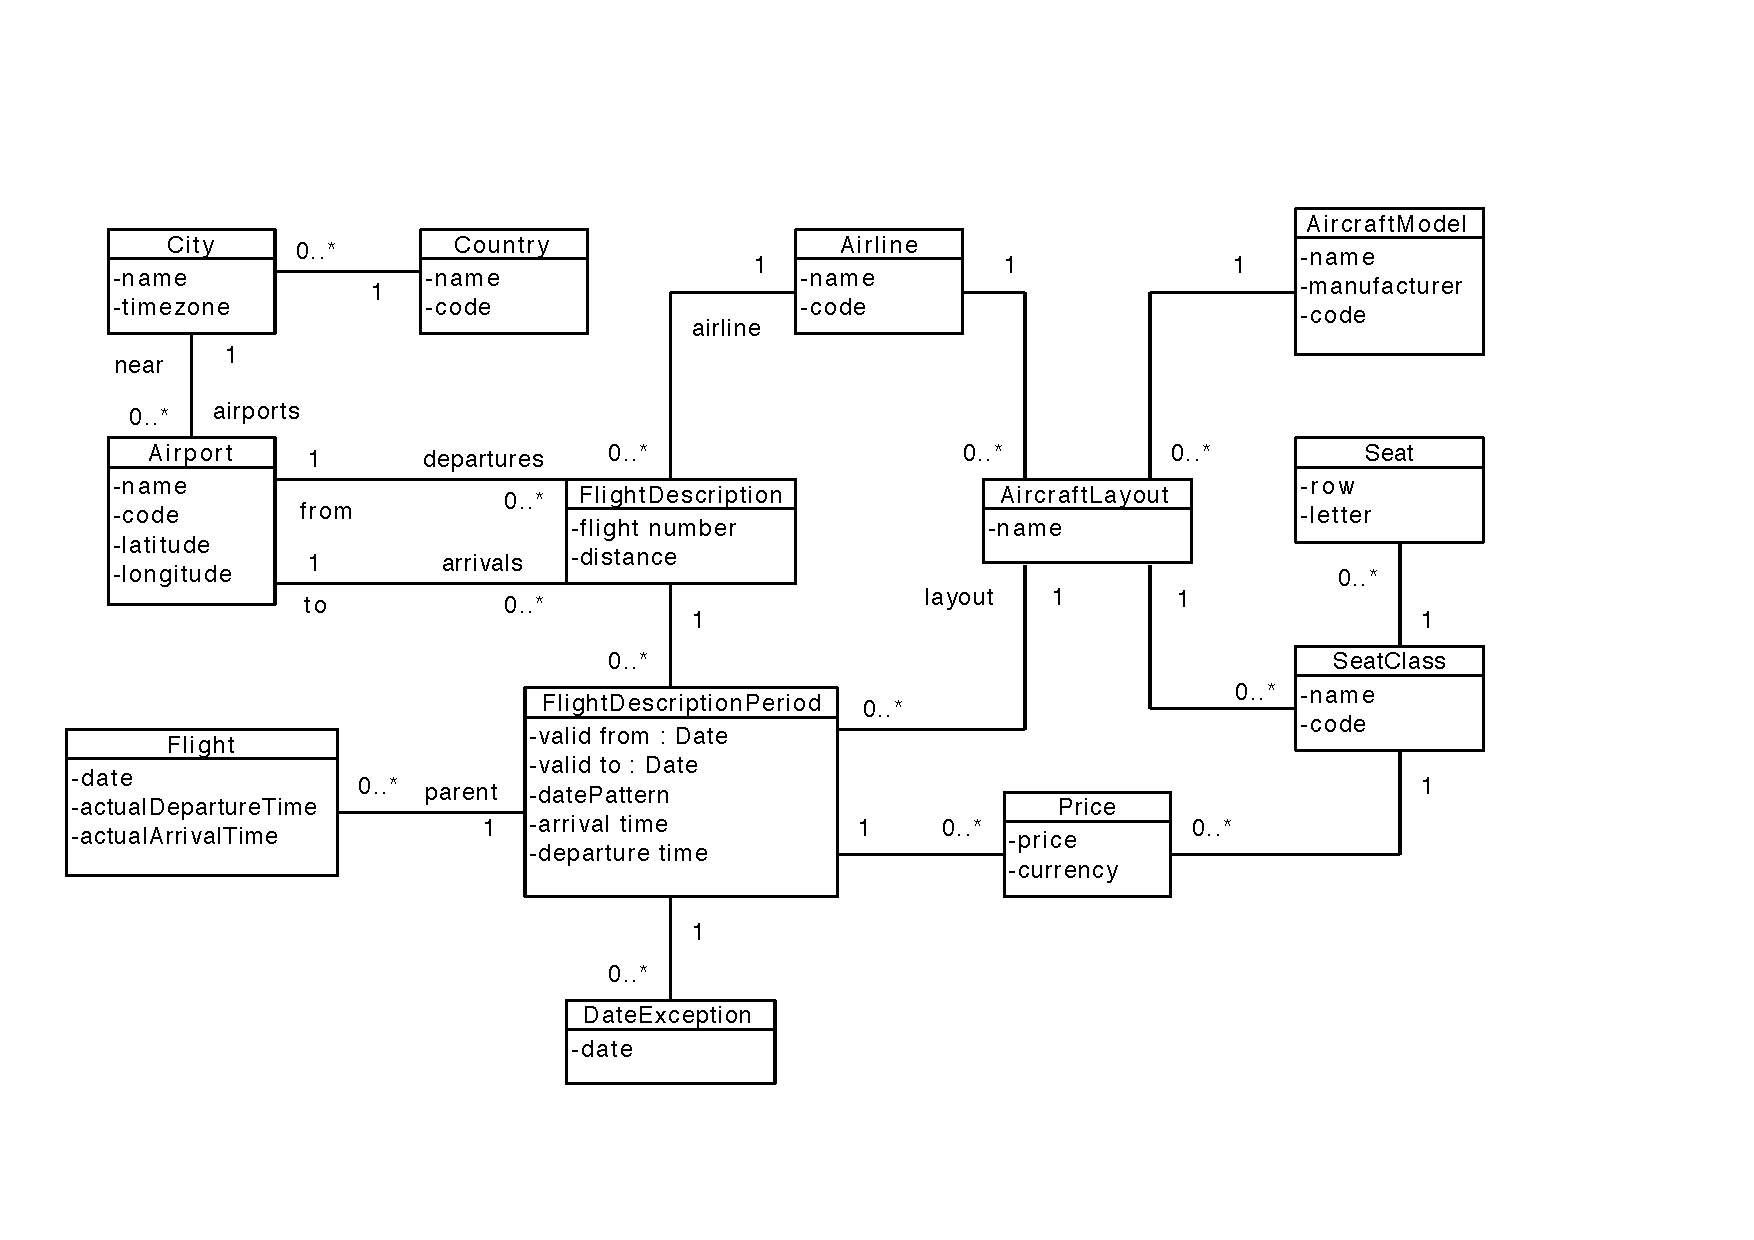
\includegraphics[width=\textwidth]{domain-model.pdf}
    \caption{Domain model}
    \label{fig:domain-model}
\end{figure}

\subsection{Additions to the domain}
\begin{itemize}
\item The concept \dsltype{AircraftLayout} is added to the domain because an \dsltype{Airline} is free to customize the seat layout of a certain \dsltype{Aircraft}. For example, one airline can make all the seats at the second level of the Airbus A380 business class while another airline can make only half of the seats at the second level business class and the other half economy class. To make this possible in our domain, the addition of the \dsltype{AircraftLayout} concept was necessary.

\item As information about every seat needs to be recorded, we keep track of the row and the letter of a seat, as used in standard airplane seating. Furthermore, we've made a \dsltype{SeatClass} concept to denote to which class a certain seat belongs. The concept \dsltype{Seat} doesn't have a price attribute itself. Instead, the price of a seat is determined by its \dsltype{SeatClass} and \dsltype{FlightDescriptionPeriod} which gives more freedom to the users.

\item An \dsltype{Airline} is free to specify its own \dsltype{AircraftLayouts}, which in turn can have its own \dsltype{SeatClasses}, but every \dsltype{SeatClass} needs to have a unique identifier within this \dsltype{AircraftLayout}. Thanks to this concept, any kind of distinction between seats can be made. For example, a specific \dsltype{SeatClass} for seats near emergency exits can be made. Airlines will typically assign higher prices to these kinds of seats, since these seats have more leg space. The opposite holds for seats near the lavatories, since a lot of people will pass by and disturb the peace. This type of fine grained price setting wasn't possible if airlines were only allowed to classify seats to ``economy class'', ``business class'' or ``first class''.

\item Since certain \dsltype{Airlines} don't operate flights on certain days, like for example Christmas, we needed the \dsltype{DateException} concept. In a \dsltype{DateException}, the user can specify a date on which a \dsltype{Flight} won't fly, even if the date fits the \dsltype{DatePattern}.

\item Each \dsltype{Airport} has a 4 capital letter code, namely the ICAO airport code \citep{icao_airport}. This code is globally accepted as the code to use for Airports and consists of 4 capital letters. Codes consisting of 3 capital letters like the IATA code \citep{iata_airport} (used for Airports outside the United States) and the FAA code \citep{faa_airport} (used for Airports inside the United States) can contain doubles which is not desirable as the code field should be unique. This is the reason why we use the ICAO code for the airports.

\item The \dsltype{FlightDescription} and \dsltype{FlightDescriptionPeriod} concepts represent a flight template. \dsltype{FlightDescription} specifies which \dsltype{Airline} serves the flight, from which to which \dsltype{Airport} this flight goes, what flight number is attached to it and what the distance of the flight is.
\spar \dsltype{FlightDescriptionPeriod} on the other hand specifies in which period flights for this \dsltype{FlightDescription} exist, what \dsltype{AircraftLayout} is used, which \dsltype{Prices} are attached to the seats of the \dsltype{AircraftLayout} for these flights and at what time of the day these flights leave and arrive. The reason why we divided the flight template into these two concepts is that flights can have the same flight code and can be handled by the same \dsltype{Airline} but still occur in a different period, leave and arrive at a different time, flying at different days in the week and with a different \dsltype{AircraftLayout} or with the same \dsltype{AircraftLayout} but different \dsltype{Prices}.

\item Although the distance between \dsltype{Airports} can be calculated based on their latitude and longitude attributes, the user needs to manually insert the distance for a certain \dsltype{FlightDescription}. This is necessary because not all flights will fly in a straight line, which is --- obviously --- the shortest path.
\end{itemize}

\subsection{Assumptions}
\begin{itemize}
\item We assume that a flight number will not be reused for a flight that has a different route than the original flight that was associated with this flight number. In other words, flight numbers describe a certain route for a certain airline and hence the combination ``airline -- flight number'' is unique.

\item We assume all dates and times are given by the users in local time, the timezone is saved in the City concept. This means that the duration of a flight is recorded implicitly: it can be calculated based on the given departure and arrival time and the time zones of the arrival and departure airports, obtained through its city.

\item As stated by the domain expert, connections of flights are not taken into account. However, since each of these flights are avaialable in the database individually, it is still possible to search for connections manually.

\item We assume that only direct flights exist, i.e. a flight will never have one or more intermediate stops. Note that this is something else than a ``connection'': in a connection, there will exist one or more stand-alone flights where each of these flights has its own flight number. If a flight has one or more intermediate stop(s), it lands at certain airport(s), refuels, drops off and picks up people, and then flies further under the same (!) flight number to its destination.

\item We assume that each flight belongs to only one airline. Or, in other words, we assume that codeshares don't exist. In a codeshare, two or more airlines will sell tickets for the same flight, but each of these airlines will assign a its own flight number (or code) to this flight. A seat can thus be purchased via multiple airlines, while the actual flight will be operated by only one airline.
\end{itemize}

\newpage
\section{Domain Analysis}

\begin{description}
\item[Country]
A \dsltype{Country} has a \dslattr{name} and a unique ISO-\dslattr{code} of 2 letters \citep{iso_country}. A \dsltype{Country} can have any number of \dsltype{Cities}.

\item[City]
A \dsltype{City} has a \dslattr{name} and \dslattr{timezone}. As said above, the timezone attribute is needed to calculate the duration of a \dsltype{Flight}. \dsltype{Cities} are located in a \dsltype{Country} and can have any number of \dsltype{Airports}.

\item[Airport]
An \dsltype{Airport} has a \dslattr{name}, a unique 4-letter ICAO-\dslattr{code}, a \dslattr{latitude} and \dslattr{longitude} attribute.
\spar The latitude and longitude attributes are used to specify the exact location of the \dsltype{Airport}, but are not used to calculate the distance between airports because flights usually don't fly in a straight line. An \dsltype{Airport} can have any number of \dsltype{FlightDescriptions} using the \dsltype{Airport} as departure or destination \dsltype{Airport}.

\item[AircraftModel]
An \dsltype{AircraftModel} has a \dslattr{name}, a \dslattr{manufacturer} and a unique ICAO-\dslattr{code}. An \dsltype{AircraftModel} can have any number of \dsltype{AircraftLayouts}.

\item[Airline]
An \dsltype{Airline} has a \dslattr{name} and a unique 3-letter ICAO-\dslattr{code} attribute. An \dsltype{Airline} can have any number of \dsltype{AircraftLayouts} and serve any number of \dsltype{FlightDescriptions}.

\item[AircraftLayout]
An \dsltype{AircraftLayout} has a \dslattr{name} which has to be unique for the \dsltype{Airline} it belongs to. \dsltype{AircraftLayout} also references its \dsltype{Airline} (by its ICAO-code) and its \dsltype{AircraftModel} (its ICAO-code). An \dsltype{AircraftLayout} contains a number of \dsltype{SeatClasses} and can serve any number of \dsltype{FlightDescriptionPeriods}.

\npar As said in the domain description, an \dsltype{AircraftLayout} describes the seating layout for a specific \dsltype{AircraftModel} and \dsltype{Airline} because not every \dsltype{AircraftModel} has the exact same layout.

\item[SeatClass]
A \dsltype{SeatClass} has a \dslattr{name} and a self-chosen \dslattr{code} that has to be unique for its \dsltype{AircraftLayout} but not globally unique. A \dsltype{SeatClass} references its \dsltype{AircraftLayout} and can have any number of \dsltype{Prices} and \dsltype{Seats}.

\item[Seat]
A \dsltype{Seat} is determined by a \dslattr{row} and a \dslattr{letter}. The combination of these two has to be unique for each \dsltype{AircraftLayout}. A \dsltype{Seat} contains references to its \dsltype{SeatClass} (by its code).

\item[FlightDescription]
A \dsltype{FlightDescription} has a \dslattr{flight number} and a \dslattr{distance}. A \dsltype{FlightDescription} references the \dsltype{Airline} (ICAO-code) which serves the flights generated from this description and two \dsltype{Airport} identifiers (ICAO-codes), representing the departure and the arrival \dsltype{Airport}. A \dsltype{FlightDescription} can also have any number of \dsltype{FlightDescriptionPeriods}. The combination of the \dsltype{Airline} identifier and the flight number has to be unique.

\item[FlightDescriptionPeriod]
A \dsltype{FlightDescriptionPeriod} describes a period in which a certain \dsltype{FlightDescription} is valid. It has a start date (\dslattr{valid from}), an end date (\dslattr{valid to}), a \dslattr{datePattern} and the \dslattr{arrival time} and \dslattr{departure time} in that period. A \dsltype{FlightDescriptionPeriod} references an \dsltype{AircraftLayout} which will serve the flights described by this period. A \dsltype{FlightDescriptionPeriod} can also have any number of \dsltype{Prices}, \dsltype{DateExceptions} and \dsltype{Flights}.

\npar The time of the start date and end date is set to midnight. The datePattern is a bitmask that contains a boolean for every day of the week, each specifying whether a flight exists on that day. These seven booleans are saved as an integer in the database. The arrival time and departure time are saved as date objects as well with the date of the objects set to epoch. The date of the arrival time can be different from epoch when the flight arrives a day (or two days maximum) after the flight left. This difference arises for example when a flight departs at 23:00 and arrives the following day.

\begin{center}
\begin{tabular}{l|l}
If this is true & this day of the week is included \\
\hline
(datePattern \& (1 << 0)) != 0 & Sunday \\
(datePattern \& (1 << 1)) != 0 & Monday \\
(datePattern \& (1 << 2)) != 0 & Tuesday \\
(datePattern \& (1 << 3)) != 0 & Wednesday \\
(datePattern \& (1 << 4)) != 0 & Thursday \\
(datePattern \& (1 << 5)) != 0 & Friday \\
(datePattern \& (1 << 6)) != 0 & Saturday \\
\end{tabular}
\end{center}

\item[Flight]
A \dsltype{Flight} describes an actual flight. It has a \dslattr{date}, an \dslattr{actualDepartureTime} and an \dslattr{actualArrivalTime} attribute. A \dsltype{Flight} references the \dsltype{FlightDescriptionPeriod} from which it is created.

\npar In the actualDepartureTime and the actualArrivalTime attributes of \dsltype{Flight}, the theoretical departure time and arrival time of FlightDescriptionPeriod can be overridden to represent, respectively, the actual departure and arrival time as a result of potential delays or advances. The date of actualDepartureTime is set to epoch but can deviate from it when for example the flight was planned at 23:50 but had 20 minutes of delay, then the actualDepartureTime will be 2 january 1970 00:10. The date of actualArrivalTime is set to epoch as well but can deviate from it when the flight had a delay or the plane arrives a day (or two days maximum) after it left.
\par The departureTime cannot account for planes departing the day before, e.g. it's scheduled to depart at 00:10 but departs 11 minutes too early. In this case, the user will have to decide to either take 00:00 as departure time, or keep the theoretical time. There is no problem with planes arriving a day too early, because this can only mean that the theoretical arrival time has a +1 (or more), which can be left out (or lowered).

\item[DateException]
A \dsltype{DateException} describes on which explicit \dslattr{dates} a flight won’t fly even if its datePattern fits the date.

\item[Price]
A \dsltype{Price} describes the \dslattr{price}, given in a certain \dslattr{currency} for a certain \dsltype{SeatClass} on a flight in a certain \dsltype{FlightDescriptionPeriod}. This allows airlines to have different prices for some seat class for the same flight but in different periods.

\end{description}

\newpage
\section{Design description}
The syntax of the DSL is the following:
\begin{quote}
\begin{verbatim}    
Type{ arguments }.SubType{ arguments }		
Type{ arguments }
\end{verbatim}
\end{quote}

We've decided to name all arguments. This means that the order of the arguments doesn't matter. \dslcode{Country\{ name: ``Belgium'', code: ``BE'' \}} is the same as \dslcode{Country\{ code: ``BE'', name: ``Belgium'' \}}. The way the parameters are named is the same as in JSON, apart from the fact that the parameter names don't have to be quoted.

The different subtypes can be chained, e.g.
\begin{quote}\begin{verbatim}
Type{ args }.SubType{ args }.SubSubType{ args }
\end{verbatim}\end{quote}

Chaining also allows going back to a type mentioned before, e.g.
\begin{quote}\begin{verbatim}
Type{ args}
   .SubType{ args }
       .SubSubType{ args }
   .SubType{ args }
\end{verbatim}\end{quote}

This is possible everywhere but the flights (see below).
An example of the DSL:
\begin{quote}\begin{verbatim}
Country{ name: "Belgium", code: "BE" }
   .City{ name: "Brussels", timezone: "Europe/Brussels" }
       .Airport{ name: "Brussels Airport" /* ... */ }
   .City{ name: "Charleroi", timezone: "Europe/Brussels" }
       .Airport{ name: "Brussels South Airport (Charleroi)" /* ... */ }
\end{verbatim}\end{quote}

This small DSL describes the country Belgium with two cities, Brussels and Charleroi, which each have one airport, respectively Brussels Airport and Brussels South Airport (Charleroi).

\npar The DSL can be commented, using the same syntax as all C-based languages:
\begin{quote}\begin{verbatim}
// a single line of comment
Country{ name: "Belgium", code: "BE" } // comment after code
/* this
is
a
multiline
comment */
\end{verbatim}\end{quote}

\clearpage
\section{Implementation overview}

\paragraph*{Why JavaScript?} The syntax of the DSL closely resembles the JSON notation. Because the quotes surrounding the attribute names can be omitted, the notation also closely resembles the JavaScript notation for describing objects. This is one of the reasons we've decided to implement our DSL in JavaScript.
\par Another reason to use JavaScript is the flexibility of the language. It has dynamic typing and does not do any consistency checking on the objects or functions being called. If a parameter does not exist, an error will eventually be thrown if the program tries to access it in a certain way. The fact that missing or extra parameters don't result in syntax errors like they would in many other compiled languages allows the implementation to handle these kinds of errors in the DSL.
\par A minor advantage of using JavaScript is that we all have experience with the language. Other possible host languages we looked at include Ruby, Perl and Python, but our knowledge of these languages is basic at best.

\paragraph*{Implementation details} We have chosen to use the node.js JavaScript environment. We've chosen node because it has a powerful code evaluator which allows us to actually run the files the user has given us. Another advantage of node is the node package manager, which contains hundreds of extensions, e.g. packages for SQLite and PostgreSQL.
\par To run, we create a scope and run the DSL sandboxed in this scope. The DSL syntax is very closely related to JavaScript. To be able to run the DSL, only a couple of regular expressions are needed to create valid JavaScript code from the input file.
\par We use an Object-Relational Mapper (ORM) and DataBase Abstraction Layer (DBAL) to communicate with the database. This allows us to work with objects instead of creating the SQL ourselves and make abstraction of which kind of database is used. The user can use whichever type of daatabase he or she prefers, as long as the DBAL supports it. The supported databases are MySQL, PostgreSQL and SQLite.

\par In general, one JavaScript object will be created and persisted per \dslcode{Type\{ arguments \}} call in the DSL. The only exceptions are when the object already exists, and the \dsltype{Flight} object. The \dsltype{Flight} objects are automatically generated when the line describing the \dsltype{FlightDescriptionPeriod} they belong to is created.
The \dslcode{Flight\{ arguments \}} calls are only allowed to follow a \dslcode{FlightDescription\{ arguments \}} call, a previous \dslcode{Flight\{ arguments \}} call, or they can be a starting call.
This implies that \dslcode{Flight\{ arguments \}} calls are only permitted in lines below the one where they're created, as a \dsltype{FlightDescriptionPeriod} is required before \dsltype{Flights} are created.

\begin{quote}\begin{verbatim}
// Let's assume flight BRU0001 has already been created before.

// This works
FlightDescription{ airline: "BRU", flightNumber: 0001 }
   .Flight{ date: "11 jan 2013", actualArrivalTime: "00:20+1" }
   .Flight{ date: "12 jan 2013", actualArrivalTime: "00:21+1" }
Flight{ airline: "BRU", flightNumber: 0002 }
   .Flight{ date: "13 jan 2013", actualArrivalTime: "00:22+1" }

// This doesn't work
FlightDescription{ airline: "BRU", flightNumber: 0001 }
   .Period{ /* ... */ }
   .Flight{ /* ... */ }
\end{verbatim}\end{quote}

A call to \dslcode{Type\{ arguments \}} is not guaranteed to create an object. If the object it describes already exists, that object is returned instead. This enables the user to re-use defined objects by simply calling \dslcode{Type\{ idArgument: value \}}, where \dslattr{idArgument} is an identifying argument.

\spar Examples:
\begin{quote}\begin{verbatim}
// Create the country Belgium
Country{ name: "Belgium", code: "BE" }
Country{ code: "BE" } // is the same country as above
Country{ name: "Belgium" } // is the same country as above
\end{verbatim}\end{quote}

Using this with only the identifying variable given is supported, but will result in an error if the object does not exist yet.

\spar Any extra arguments will be verified when the object exists already. This is because the program doesn't know which country the user wants in the second line of this example:
\begin{quote}\begin{verbatim}
Country{ name: "Belgium", code: "BE" }
Country{ name: "France", code: "BE" }
\end{verbatim}\end{quote}

Both \dslattr{name} and \dslattr{code} are identifiers of a \dsltype{Country}. The second line in the previous example results in two different \dsltype{Countries} depending on which id is checked first. Because of that, the program will return an error.

\par When a non-identifying property is given and differs from the value of the already existing object with the same identifier(s), the program will also return an error. We've opted to not silently ignore this, because we don't know if the user made a mistake or wants to update. Updates are not supported, and if the user makes a mistake, we don't know if the mistake was made in the identifying variable or in the other variable.
\par The only exception to this rule is the \dslcode{Flight\{ arguments \}} call. This does update the \dslattr{actualArrivalTime} and \dslattr{actualDepartureTime} arguments if they're given. This is because the \dsltype{Flight} objects are not created because the user called \dslcode{Flight\{ arguments \}}. Upon creation of a \dsltype{FlightDescriptionPeriod} object, all \dsltype{Flight} objects for that period are created with the theoretical departure and arrival times. The user can change this times by giving another time.

\paragraph*{Errors} Any error that the program encounters will be shown to the user. The exact location of the error is unknown, because the regular expressions described above add extra characters to every line. However, as the line number is not changed, this is shown to the user. The error itself contains a description of what is wrong, e.g. ``MissingAttributeError: row not set for seat'' or ``InvalidArgumentError: aircraft model with code  A388 doesn't exist''.
\par The following error types exist, apart from syntax errors in the DSL files and any database issues that may arise:
\begin{quote}\begin{description}
\item[InvalidArgumentError] All errors below are subtypes of this error type. It denotes a problem with the arguments in one of the DSL calls.
\item[DuplicateError] The DSL is trying to create an object with an identifier that has already been used.
\item[DataMismatchError] The DSL descibes an object that already exists, but some attributes of the object are different.
\item[MissingAttributeError] Some attributes of a DSL call are mising.
\item[ValidationError] An attribute has an invalid value, e.g. a four-letter alphanumerical string where a two-letter alpha string was expected.
\end{description}\end{quote}

\clearpage
\section{DSL implementation}

Our DSL implementation depends on a couple of libraries, depending on which database is used. An obvious dependency is node.js. We developed the DSL using version 0.8.16, which is the target version, but later versions should work as well.
We use an ORM/DBAL, cf supra. We've decided to use Sequelize \citep{sequelize}. We've used the latest version, which is 1.6.0-beta4, but future 1.6.x versions should work as well.
Depending on which database is actually used, the program depends on the sqlite, pg or mysql node modules and the corresponding packages on the computer itself.

\npar The code of the program works in three steps, loading the database, creating the object structure for the DSL and storing the data.
\par The main reason for the split between evaluating the DSL and storing the data is two-fold. We don't use any transactions in the ORM, so if an error occurs when half of the data has been saved, we don't have a way to rollback.
\par The other reason is also the reason why we first load the database. All interactions with the database are asynchronous. This results in unforseen and unpredictable problems. One example is the following: Country A is created, and city \(C_A\) is added. Then, country B is created and city \(C_B\) is added. After running this DSL, the database would list both \(C_A\) and \(C_B\) as being cities in country B. This is because of the way Sequelize adds elements in a one-to-many relation. Another example is simply that the DSL could require a country to exist in the database, but the database is still being read.

\npar We decided to load the preexisting data from the database, to allow the user to add new elements to existing data. It is also possible to run the program with multiple DSL files. The program will then load the database after which it will run all the DSL files one by one in the order given and finally it stores the result. This means that nothing will be stored if e.g. the third file contains an error.

\paragraph*{Consistency checks} A number of consistency checks are included. When \dslcode{Type\{ arguments \}} is called, it is checked whether all the expected arguments are present. The type and format of the arguments are checked before they are saved in the database and thus the user also receives errors if the format or type is incorrect. As JavaScript allows a user to give extra arguments to a method without checking them, the user of the DSL could for example use the following code: \dslcode{Country\{ name: "Belgium", code: "BE", king: "Albert II" \}} in which the argument ``king'' is completely ignored.
Furthermore if an attribute references an object that doesn't exist, e.g. a \dsltype{AircraftLayout} with an unexistent \dsltype{Airline}Id, an InvalidArgumentError will be thrown. When the reference is correct but in the rest of the attributes differs from the preexisting object, a DataMismatchError will be thrown.

\paragraph*{Future extensions} Because we don't use a parser to interpret the syntax, the DSL can be extended pretty easily. As explained above, the only modifications that are needed to add an attribute to an existing concept are (1) the definition of the attribute in the database schema (db.js) and (2) a modification in the creator function of the corresponding concept. 
\par When a concept is added on the other hand, there are two options. Either the concept is a top level concept (this is a concept from which elements can be created without the use of other elements) or it is not. To add a top level concept another file must be created containing the same methods as other concept files. To add a non top level concept, the methods for this concept have to be added to the file of its ``parent'' concept.
\clearpage
\section{User guide}

\subsection{Installation}
Install node and npm (the node package manager). Download the source from the git repository (\url{https://github.com/bgotink/CPL}) or extract the tarball found with this report.
\npar Decide which database to use. The simplest to use is SQLite, but this is extremely slow on hard disks. A run time of one hundred seconds is to be expected even for pretty small files, while a solid state disk results in a run time of one second.
\par Edit src/package.json, remove the database dependencies for the databases you won't use. The three types are: sqlite3, pg and mysql. You don't have to remove the unneeded libraries, but trying to install the node packages could result in errors if the real programs and their libraries are not installed on the computer.
\npar Next, run \texttt{npm install} in the src-directory of the DSL. This will install all dependencies described in the package.json file.

\npar An alternative way to install the dependencies is to run \texttt{make install} in the root directory of the DSL project. This will only work if node, npm and the necessary database packages are installed on the computer.

\subsection{Configuration}
The file src/config.js must be created to configure the program. This file tells the program what to log and which database to use. The file src/config.js.dist contains all the options the user can change, and shows how to create every type of database. Simply copying this file to src/config.js will make the program use a SQLite database in data/db.sqlite.

\subsection{Execution}
First, open a terminal and go to the main directory of the program (containing subdirectories src, test, data \ldots). Once there, you can start the program using:
\begin{quote}\begin{verbatim}
node src/dsl.js <inputfile> [inputfile ...]
\end{verbatim}\end{quote}

\npar To run some testfiles, \texttt{make test} can be used in the head directory to run a test DSL file. Running \texttt{make test\_long} will run all tests, and one extra big file, which can take several minutes to store.

\clearpage
\bibliography{report}

\clearpage
\appendix
\section{DSL API}
In this section, we'll give an overview of all the language constructs of our DSL. Attributes with an asterisk (*) are unique identifiers, attributes with a tilde (\mytilde) have a note below.

\subsection*{Country - City - Airport}
Here, the language constructs and the sequence of these constructs for adding an airport to a certain city will be shown. First, the sequence of these constructs will be shown by using an abbreviated notation of the constructs. Thereafter, each language construct will be shown in full (with all his parameters).

\subsubsection*{Add an airport to a certain city}
\begin{tabbing}
Country \= \{\ldots \} \\
\> .City \= \{\ldots \} \\
\> \> .Airport \= \{\ldots \} \\
\end{tabbing}

\subsubsection*{Add a country}
\begin{tabbing}
Country \= \{ \= name*: "\textit{name of the country}", \\
	\> \> code*: "\textit{code of the country}" \\
\> \} \\
\end{tabbing}

\subsubsection*{Add a city}
\begin{tabbing}
.City \= \{ \= name\mytilde: "\textit{name of the city}", \\
	\> \> timezone: \= "\textit{timezone of the city}" \\
    \> \> \> (See: \nameref{Timezone}) \\
\> \} \\
\end{tabbing}
Notes:
\begin{enumerate}
\item[name] The name is unique within the \dsltype{Country}.
\end{enumerate}

\subsubsection*{Add an airport}
\begin{tabbing}
.Airport \= \{ \= name: "\textit{name of the airport}", \\
	\> \> code*: "\textit{code of the airport}", \\
	\> \> longitude: "\textit{longitude of the airport}", \\
	\> \> latitude: "\textit{latitude of the airport}" \\
\> \} \\
\end{tabbing}

\subsection*{Airline - AircraftModel - AircrafLayout - SeatClass - Seat}
Here, the language constructs and the sequence of these constructs for adding a seat of certain seat class in an aircraft layout of an airline will be shown. First, the sequence of these constructs will be shown by using an abbreviated notation of the constructs. Thereafter, each language construct will be shown in full (with all his parameters).

\subsubsection*{Add a seat of a certain seat class to the aircraft layout of an airline}
\begin{tabbing}
AircraftModel \= \{\ldots \} \\

Airline \= \{\ldots \} \\
\> .AircraftLayout \= \{ \ldots \} \\
\> \> .SeatClass \= \{ \ldots \} \\
\> \> \> .Seat \= \{ \ldots \} \\
\end{tabbing}

\subsubsection*{Add an AircraftModel}
\begin{tabbing}
AircraftModel \= \{ \= name: "\textit{name of the aircraft model}", \\
	\> \> manufacturer: "\textit{manufacturer of the aircraft model}", \\
	\> \> code*: "\textit{code of the aircraft model}" \\
\> \} \\
\end{tabbing}

\subsubsection*{Add an Airline}
\begin{tabbing}
Airline \= \{ \= name: "\textit{name of the airline}", \\
	\> \> code*: "\textit{code of the airline}" \\
\> \} \\
\end{tabbing}

\subsubsection*{Add an AircraftLayout}
\begin{tabbing}
.AircraftLayout \= \{ \= name\mytilde: "\textit{name of the aircraft layout}", \\
	\> \> modelCode: "\textit{code of the aircraft model}" \\
\> \} \\
\end{tabbing}
Notes:
\begin{enumerate}
\item[name] The name is unique for that \dsltype{Airline}.
\end{enumerate}

\subsubsection*{Add a SeatClass}
\begin{tabbing}
.SeatClass \= \{ \= name: "\textit{name of the seat class}", \\
	\> \> code\mytilde: "\textit{code of the seat class}" \\
\> \} \\
\end{tabbing}
Notes:
\begin{enumerate}
\item[code] The code is unique for that \dsltype{AircraftLayout}.
\end{enumerate}

\subsubsection*{Add a Seat}
\begin{tabbing}
.Seat \= \{ \= row\mytilde: "\textit{row of the seat}", \\
	\> \> letter\mytilde: "\textit{letter of the seat}" \\
\> \} \\
\end{tabbing}
Notes:
\begin{enumerate}
\item[row]
\item[letter] The combination of row and letter has to be unique for the \dsltype{AircraftLayout} this seat belongs to. This implies that the combination is also unique for the \dsltype{SeatClass}.
\end{enumerate}

\subsection*{FlightDescription - FlightDescriptionPeriod - DateException - Price}
Here, the language constructs and the sequence of these constructs for adding a flight template (consisting of a flight descprition, a period with exceptions and prices) will be shown. First, the sequence of these constructs will be shown by using an abbreviated notation of the constructs. Thereafter, each language construct will be shown in full (with all his parameters).

\subsubsection*{Add a flight template}
\begin{tabbing}
FlightDescription \= \{\ldots \} \\
\> .FlightDescriptionPeriod \= \{ \ldots \} \\
\> \> .DateException \= \{ \ldots \} \\
\> \> .Price \= \{ \ldots \} \\
\> \> .Price \= \{ \ldots \} \\
\> \> .DateException \= \{ \ldots \} \\
\end{tabbing}

Note that the language constructs \dsltype{DateException} and \dsltype{Price} both operate on a certain \dsltype{FlightDescriptionPeriod} and are interchangeable.

\subsubsection*{Add a FlightDescription}
\begin{tabbing}
FlightDescription \= \{ \= flightNumber\mytilde: "\textit{number of the flight descprtion}", \\
	\> \> distance: \textit{distance between departure and arrival airport}, \\
	\> \> from: "\textit{code of the departure airport}", \\
	\> \> to: "\textit{code of the destination airport}", \\
	\> \> airline: "\textit{code of the airline}" \\
\> \} \\
\end{tabbing}
Notes:
\begin{enumerate}
\item[flightNumber] The flightNumber is unique for that \dsltype{Airline}.
\end{enumerate}

\subsubsection*{Add a FlightDescriptionPeriod}
\begin{tabbing}
.FlightDescriptionPeriod \= \{ \= validFrom\mytilde: \= "\textit{startdate of period}", \\
		\> \> \>(See: \nameref{Date}) \\
	\> \> validTo: \= "\textit{enddate of period}", \\
		\> \> \>(See: \nameref{Date}) \\
	\> \> datePattern\mytilde: \= "\textit{date pattern of the period}", \\
		\> \> \>(See: \nameref{Datepattern}) \\
	\> \> departureTime: \= "\textit{theoretical departure time of the flight in this period}", \\
		\> \> \>(See: \nameref{Time}) \\
	\> \> arrivalTime: \= "\textit{theoretical arrival time of the flight in this period}", \\
		\> \> \>(See: \nameref{Time}) \\
	\> \> aircraftLayout: "\textit{name of the aircraft layout}" \\
\> \} \\
\end{tabbing}
Notes:
\begin{enumerate}
\item[validFrom]
\item[datePattern] The combination of validFrom and datePattern is unique for the \dsltype{FlightDescription}.
This allows the airline to have two separate pricings for different days for the same flight in the same time period.
\end{enumerate}

\subsubsection*{Add a DateException}
\begin{tabbing}
.DateException \= \{ \= date\mytilde: \= "\textit{date of the date exception}" \\
        \> \> \>(See: \nameref{Date}) \\
\> \} \\
\end{tabbing}
Notes:
\begin{enumerate}
\item[date] The date is unique for the \dsltype{FlightDescriptionPeriod}.
\end{enumerate}

\subsubsection*{Add a Price}
\begin{tabbing}
.Price \= \{ \= price: "\textit{amount of the price}", \\
	\> \> currency: "\textit{currency of the price}", \\
	\> \> seatClass\mytilde: "\textit{seat class for this price}" \\
\> \} \\
\end{tabbing}
Notes:
\begin{enumerate}
\item[seatClass] There is exactly one \dsltype{Price} object for every \dsltype{SeatClass} for the \dsltype{AircraftLayout} used in the \dsltype{FlightDescriptionPeriod}.
\end{enumerate}

\subsection*{Flight}
Flight is an exceptional concept because it is automatically generated and thus users can not add Flights themselves. The constructs that are given below can only update the flight data in the database but cannot create new flight instances.
There are two ways to update flight data:

\begin{tabbing}
Flight \= \{ \= airline: "\textit{the code of the airline}", \\
	\> \> flightNumber: "\textit{flightNumber}", \\
	\> \> date: \= "\textit{date of the flight}", \\
        \> \> \>(See: \nameref{Date}) \\
	\> \> actualDepartureTime: \= "\textit{new departure time of the flight}", \\
        \> \> \>(See: \nameref{Time}) \\
	\> \> actualArrivalTime: \= "\textit{new departure time of the flight}" \\
        \> \> \>(See: \nameref{Time}) \\
\> \} \\

or
\end{tabbing}

\begin{tabbing}
FlightDescriptionPeriod \= \{ \= flightNumber: "\textit{flightNumber}", \\
	\> \> airline: "\textit{the code of the airline}" \\
\> \} \\
\> .Flight \= \{ \= date: \= "\textit{date of the flight}", \\
        \> \> \> \> (See: \nameref{Date}) \\
	\> \> actualDepartureTime: \= "\textit{new departure time of the flight}", \\
        \> \> \>(See: \nameref{Time}) \\
	\> \> actualArrivalTime: \= "\textit{new departure time of the flight}" \\
        \> \> \>(See: \nameref{Time}) \\
\> \} \\
\end{tabbing}


\subsection*{Usage of non-trivial attributes}
\subsubsection*{Timezone: [String]}
\label{Timezone}
A timezone has to be given as a valid tz timezone, all the valid timezones can be found here: \url{http://en.wikipedia.org/wiki/List_of_tz_database_time_zones}.

\subsubsection*{Date: [Date]}
\label{Date}
A normal date has to be given as a string either in the format ``dd mmm yyyy'' or in the ISO 8601 format ``yyyy-mm-dd''. \newline
	For example: ``07 jan 1997'' or ``1997-01-07''
	
\subsubsection*{Date pattern: [String]}
\label{Datepattern}
A date pattern has to be given as a comma separated sequence of days, spaces are ignored. Days can be given with their full name (e.g. monday) or with the abbreviation (e.g. mon) using either uppercase or lowercase. The list of possible entries is: ``monday, tuesday, wednesday, thursday, friday, saturday, sunday'' or ``mon, tue, wed, thu, fri, sat, sun''. \newline
For example: ``mon, wed, fri''


\subsubsection*{Time: [String]}
\label{Time}
A normal time has to be given as a string in the following format: ``hh:mm + d'' with d being the difference in days between the departure date and the arrival date. Spaces are ignored. \newline
For example: ``01:30 +1''

\end{document}


